\chapter{Introduction}
\label{chap:introduction}

\section{Background}
\label{section:background}

In large campuses or complexes with multiple departments or offices within the same area, parking often becomes a common inconvenience for commuters.
Many individuals waste time driving to a parking lot close to their destination, only to find their preferred lot full, forcing them to look for parking elsewhere. This can potentially add unnecessary stress to individual days.


Kasetsart University's Bangkhen Campus spans 1,356,800 square meters and houses 18 faculties, 3 colleges, 3 institutes, 6 divisions/offices, and 6 centers/institutes \cite{ku_campus_info}. With constant traffic of students, employees, visitors, and the general public, the campus experiences persistent parking challenges due to scattered parking lots and limited parking availability. This issue is even more frustrating for non-resident visitors unfamiliar with the area, such as those navigating Kasetsart University, where finding available parking can be particularly challenging without prior knowledge of the area layout. The complexity is further compounded by the road system, which consists of multiple one-way streets, making it difficult for drivers to efficiently navigate between parking areas and forcing them into longer detours when the preferred parking is not available.


Many parking facilities address this challenge by installing parking indicators that display the number of available spots or highlight specific vacant spaces.
These systems help users determine parking availability before entering the lot, reducing unnecessary driving time and congestion. However, they typically rely on sensors installed in individual parking spots to detect occupancy.
While effective, such sensor-based systems require significant installation and maintenance costs.
As a result, many parking owners choose not to implement these systems due to budget constraints, leaving drivers to search for parking without any indicator.

\section{Problem Statement}
\label{section:problem-statement}
The problem addressed by KU Parking is that commuters on campus struggle to find available parking without having to drive around. Due to limited information about parking availability and, in some cases, unfamiliarity with the area, drivers often waste significant time, leading to individual frustration. 

The implementation of a parking indicator system can be costly and impractical, as the installation and financial constraints may not suit campuses or complexes with multiple parking lots spread across the area. Additionally, existing image-based systems are typically implemented on single parking lots, lacking integration between multiple parking areas. Furthermore, there is no accessible platform, such as a mobile app, for drivers to easily gain real-time information about parking availability across the entire.

\section{Solution Overview}
\label{section:solution-overview}

KU-Parking is a system consisting of two main components: the parking detection system and the mobile application. The parking detection system uses existing surveillance cameras or portable camera modules to monitor parking spaces and processes the camera feeds through cloud-based computer vision. It integrates YOLO for vehicle detection and uses Intersection over Union (IoU) calculations to determine occupancy. The mobile application provides users with parking availability information, guiding them directly to vacant spots, without the need for additional infrastructure installation.

\subsection{Features}
\label{subsection:features}

\begin{enumerate}[leftmargin=80pt]
    % TODO: to be update just a place holder
    \item Real-time Occupancy Detection: Identifies vacant and occupied parking spots using computer vision and IoU analysis.
    
    \item Cloud-based Image Processing: Analyzes camera feeds through remote servers, enabling efficient vehicle detection without requiring powerful on-site hardware.
    
    \item Mobile Parking Area Map: Displays parking lot locations across campus with real-time availability information. Integrates with third-party mapping services like Google Maps for turn-by-turn navigation to available parking areas.
    
    \item No Additional Installation Required: Utilizes existing surveillance cameras already installed throughout campus, eliminating the need for additional sensors or hardware.
\end{enumerate}

\section{Target User}
\label{section:target-user}

Our primary target users are drivers navigating to the Kasetsart University campus, particularly those unfamiliar with the campus parking facilities. Specifically:
\begin{enumerate}[leftmargin=80pt]
\item Students: New or visiting students who are unfamiliar with parking availability patterns across campus and need efficient navigation to classes.
\item Visitors and Occasional Users: Guest lecturers, parents, alumni, event attendees, and other infrequent campus visitors who have limited knowledge of campus layout and require guidance to available parking options.
\end{enumerate}


\section{Benefit}
\label{section:benefit}

% Describe potential benefits of your solution.
The KU-Parking solution offers several significant advantages:

\begin{enumerate}[leftmargin=80pt]
    \item Time Savings: Reduces driving time by providing real-time navigation to available parking spots.
    
    \item Cost-Efficiency and Infrastructure Integration: Integrating with existing surveillance camera infrastructure rather than requiring installation of expensive dedicated parking sensors or systems.
    
    \item Improved User Experience: Eliminates the frustration and uncertainty of finding parking, enhancing the overall campus experience for students and visitors.
\end{enumerate}

\section{Timeline}
\label{section:timeline}

\begin{figure}[h!]
    \centering
    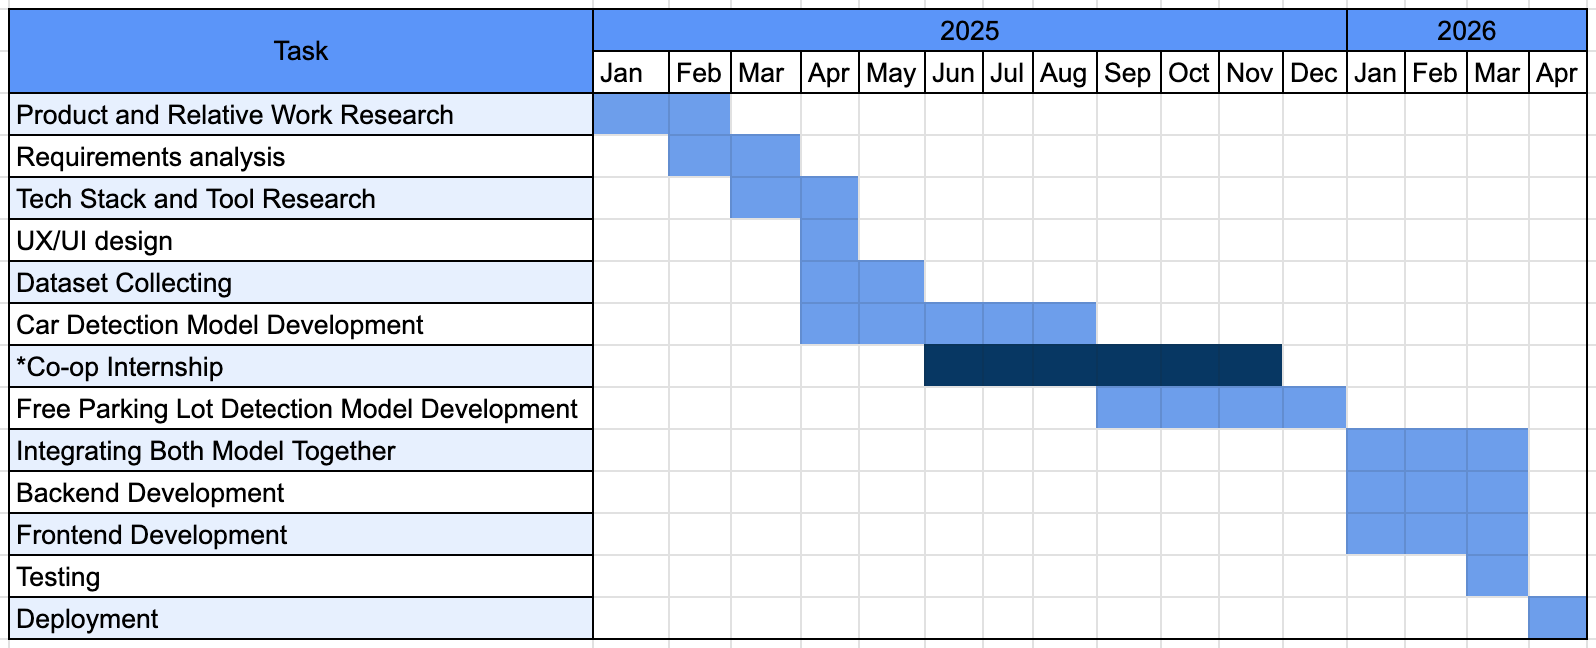
\includegraphics[width=\textwidth,height=0.5\textheight,keepaspectratio]{timeline/KU-Parking_timeline.png}
    \caption{Timeline for KU Parking Project}
    \label{fig:timeline}
\end{figure}

Figure \ref{fig:timeline} illustrates the timeline of the KU Parking Project.

The Research and Design phase began in January 2025, covering related field research, requirement analysis, and UX/UI design. The Implementation phase will commence in April 2025, focusing on the development of the Car Detection Model and the Free Parking Lot Detection Model.

Following the successful implementation of both models, the Application Development phase will start in January 2026. The system will be deployed for testing in March 2026 and fully launched in April 2026.



\section{Terminology}
\label{section:terminology}

\begin{description} 
    \item[YOLO (You Only Look Once)] A computer vision algorithm used for real-time object detection, employed in this system to identify vehicles in parking spaces.

    \item[IoU (Intersection over Union)] A metric used in computer vision to calculate the overlap between predicted and actual object boundaries, used in this system to determine parking space occupancy.   
\end{description}